%
% This is the LaTeX template file for lecture notes for EE 382C/EE 361C/EE 382N/etc.
%
% To familiarize yourself with this template, the body contains
% some examples of its use.  Look them over.  Then you can
% run LaTeX on this file.  After you have LaTeXed this file then
% you can look over the result either by printing it out with
% dvips or using xdvi.
%
% This template is based on the template for Prof. Sinclair's CS 270.

\documentclass[twoside]{article}
\usepackage{graphics}
\usepackage{tikz}
\usepackage{float}
\usetikzlibrary{arrows,automata}
\usetikzlibrary{arrows,matrix,positioning}
\setlength{\oddsidemargin}{0.25 in}
\setlength{\evensidemargin}{-0.25 in}
\setlength{\topmargin}{-0.6 in}
\setlength{\textwidth}{6.5 in}
\setlength{\textheight}{8.5 in}
\setlength{\headsep}{0.75 in}
\setlength{\parindent}{0 in}
\setlength{\parskip}{0.1 in}

%
% The following commands set up the lecnum (lecture number)
% counter and make various numbering schemes work relative
% to the lecture number.
%
\newcounter{lecnum}
\renewcommand{\thepage}{\thelecnum-\arabic{page}}
\renewcommand{\thesection}{\thelecnum.\arabic{section}}
\renewcommand{\theequation}{\thelecnum.\arabic{equation}}
\renewcommand{\thefigure}{\thelecnum.\arabic{figure}}
\renewcommand{\thetable}{\thelecnum.\arabic{table}}

%
% The following macro is used to generate the header.
%
\newcommand{\lecture}[4]{
   \pagestyle{myheadings}
   \thispagestyle{plain}
   \newpage
   \setcounter{lecnum}{#1}
   \setcounter{page}{1}
   \noindent
   \begin{center}
   \framebox{
      \vbox{\vspace{2mm}
    \hbox to 6.28in { {\bf EE 382N: Distributed Systems
                        \hfill Fall 2017} }
       \vspace{4mm}
       \hbox to 6.28in { {\Large \hfill Lecture #1: #2  \hfill} }
       \vspace{2mm}
       \hbox to 6.28in { {\it Lecturer: #3 \hfill Scribe: #4} }
      \vspace{2mm}}
   }
   \end{center}
   \markboth{Lecture #1: #2}{Lecture #1: #2}
   %{\bf Disclaimer}: {\it These notes have not been subjected to the
   %usual scrutiny reserved for formal publications.  They may be distributed
   %outside this class only with the permission of the Instructor.}
   \vspace*{4mm}
}

%
% Convention for citations is authors' initials followed by the year.
% For example, to cite a paper by Leighton and Maggs you would type
% \cite{LM89}, and to cite a paper by Strassen you would type \cite{S69}.
% (To avoid bibliography problems, for now we redefine the \cite command.)
% Also commands that create a suitable format for the reference list.
\renewcommand{\cite}[1]{[#1]}
\def\beginrefs{\begin{list}%
        {[\arabic{equation}]}{\usecounter{equation}
         \setlength{\leftmargin}{2.0truecm}\setlength{\labelsep}{0.4truecm}%
         \setlength{\labelwidth}{1.6truecm}}}
\def\endrefs{\end{list}}
\def\bibentry#1{\item[\hbox{[#1]}]}

%Use this command for a figure; it puts a figure in wherever you want it.
%usage: \fig{NUMBER}{SPACE-IN-INCHES}{CAPTION}
\newcommand{\fig}[3]{
			\vspace{#2}
			\begin{center}
			Figure \thelecnum.#1:~#3
			\end{center}
	}
% Use these for theorems, lemmas, proofs, etc.
\newtheorem{theorem}{Theorem}[lecnum]
\newtheorem{lemma}[theorem]{Lemma}
\newtheorem{proposition}[theorem]{Proposition}
\newtheorem{claim}[theorem]{Claim}
\newtheorem{corollary}[theorem]{Corollary}
\newtheorem{definition}[theorem]{Definition}
\newenvironment{proof}{{\bf Proof:}}{\hfill\rule{2mm}{2mm}}

% **** IF YOU WANT TO DEFINE ADDITIONAL MACROS FOR YOURSELF, PUT THEM HERE:

\begin{document}
%FILL IN THE RIGHT INFO.
%\lecture{**LECTURE-NUMBER**}{**DATE**}{**LECTURER**}{**SCRIBE**}
\lecture{1}{Oct 13}{Vijay Garg}{Marina Thomas}
%\footnotetext{These notes are partially based on those of Nigel Mansell.}

% **** YOUR NOTES GO HERE:

% Some general latex examples and examples making use of the
% macros follow.
%**** IN GENERAL, BE BRIEF. LONG SCRIBE NOTES, NO MATTER HOW WELL WRITTEN,
%**** ARE NEVER READ BY ANYBODY.
\section{Termination Detection and Diffusing Computation}

 It is an important problem in distributed computing to develop efficient algorithms for termination and deadlock detection. Both termination and deadlock are stable properties and therefore can be detected using any global snapshot algorithm.
\section{Diffusing Computation}
\begin{enumerate}
   \item Every process is either active or passive
   \item Initially all processes are passive except for the special process called environment.
   \item A passive process can become active only if it receives a message
    \item Only active process can send messages
    \item Once the job is done, the process becomes passive
\end{enumerate}

\begin{definition}Termination - Happens when all processes are passive and all channels are empty.\end{definition}

Algorithms for many problems can be structured as diffusing computations. For example, the shortest paths from a processor in a networkcan be structured as diffusing computations. 

Below a distributed shortest-path algorithm is used to illustrate the concepts of a diffusing computation. There are a bunch of airports and the 'special' airport is Austin. Assume that we are interested in finding the shortest path or the least cost to fly from Austin(AUS) airport to all other airports. 

Every airport maintains the cost of the shortest path from the Austin to itself as known to it currently, parent or the predecessor of itself in the shortest path from the AUS to itself.

Austin(the special airport/environment) knows how much it will take to fly to itself. Cost of flying from Austin to itself is 0.

AUS starts up the diffusing computation by sending the cost of the shortest path to be 0 using a message type path.
Austin will send ("path",0) i.e (path, cost) 

Any airport that receives a message from AUS of type path with cost c determines whether its current cost is greater than the cost of reaching AUS plus the cost of reaching from AUS to itself. If that is indeed the case, then it has discovered a path of shorter cost and it updates the cost and parent variables. Further, any such update results in messages to its neighbors about its new cost. The algorithm is shown in Figure 1.1 amd Figure 1.2. 

\begin{figure}[H]
\centering
\begin{tikzpicture}[->,>=stealth',shorten >=1pt,auto,node distance=3cm,
                    semithick]
  \tikzstyle{every state}=[text=black]

  \node[circle,draw,label=90:$\infty$]         (A)                    {$ORD$};
  \node[circle,draw,label=60:$\infty$]         (B) [right of=A] {$NYC$};
  \node[circle,draw,label=-90:$0$]         (E) [below of=A] {$AUS$};
  \node[circle,draw,label=-90:$\infty$]         (D) [below of=B] {$IAH$};
  \node[circle,draw,label=-90:$\infty$]         (C) [right of=D] {$DFW$};

  \path (A) edge              node {100}  (B)
        (E) edge              node {50}  (A)
        (C) edge              node {5} (A)
        (D) edge              node {10}  (A)
        (D) edge              node {2}  (C)
        (E) edge              node {30}  (D);
\end{tikzpicture}
\caption{Shortest route - initial state} 
\end{figure}

\begin{figure}[H]
\centering
\begin{tikzpicture}[->,>=stealth',shorten >=1pt,auto,node distance=3cm,
                    semithick]
  \tikzstyle{every state}=[text=black]

  \node[circle,draw,label=90:$37$]         (A)                    {$ORD$};
  \node[circle,draw,label=60:$137$]         (B) [right of=A] {$NYC$};
  \node[circle,draw,label=-90:$0$]         (E) [below of=A] {$AUS$};
  \node[circle,draw,label=-90:$30$]         (D) [below of=B] {$IAH$};
  \node[circle,draw,label=-90:$32$]         (C) [right of=D] {$DFW$};

  \path (A) edge              node {100}  (B)
        (E) edge              node {50}  (A)
        (C) edge              node {5} (A)
        (D) edge              node {10}  (A)
        (D) edge              node {2}  (C)
        (E) edge              node {30}  (D);
\end{tikzpicture}
\caption{Shortest route} 
\end{figure}

The initial cost at all other airports is initialized to $\infty$

When an airport(j) receives a path message, it will check

\begin{tabbing}
if \= cost[i]  + {$w_ij$} < cost [j] \\
\>then cost[j] = cost[i] + {$w_ij$};
\end{tabbing}

\begin{figure}[H]
\centering
\begin{tikzpicture}[->,>=stealth',shorten >=1pt,auto,node distance=3cm,
                    semithick]
  \tikzstyle{every state}=[text=black]

  \node[state]         (A)                    {$i$};
  \node[state]         (B) [right of=A] {$j$};

  \path (A) edge              node {$w_ij$}  (B);
\end{tikzpicture}
\end{figure}

The algorithm works fine, but no process ever knows when it is done, that is, the cost variable will not decrease further. 

How do you know that the estimate is correct? $\rightarrow$ When all processes are passive and all channels are empty.

The goal is to come up with an algorithm that can detect this termination and how we can extend the diffusing computation to detect termination.

Is this predicate stable?
All processes are passive and all channels are captured. Hence it is stable.

\subsection{Dijkstra and Scholten's Algorithm}
$P_i$ is green iff $P_i$ is passive and all its outgoing channels are empty

Then,
TERM$\hspace{1mm}\equiv$ ($P_1\hspace{1mm} is\hspace{1mm} green )\land (P_2\hspace{1mm} is\hspace{1mm} green ) \land(P_3\hspace{1mm} is\hspace{1mm} green ) \ldots \land (P_n\hspace{1mm} is\hspace{1mm} green )$

This is conjunctive predicate. 

$P_i\hspace{1mm} is\hspace{1mm} red \hspace{1mm}\equiv P_i\hspace{1mm} is\hspace{1mm} not green $

Maintain a set T st it contains all red nodes $\lor$ processes.

T= $\{\} \rightarrow$ TERM

I need to maintain this set in a distributed manner. T is going to be maintained as a spanning tree.

$root $$\equiv$$ environment$\newline
Every node is going to have a variant parent

\begin{figure}[H]
\centering
\begin{tikzpicture}[->,>=stealth',shorten >=1pt,auto,node distance=2cm,
                    semithick]
  \tikzstyle{every state}=[text=black]

  \node[state]         (A)                    {$root$};
  \node[state]         (C) [below of=A] {$b$};
  \node[state]         (B) [left of=C] {$a$};
  \node[state]         (D) [right of=C] {$c$};
  \node[state]         (E) [below of=B] {$d$};


  \path (C) edge              node {}  (A)
        (B) edge              node {}  (A)
        (D) edge              node {} (A)
        (E) edge              node {} (B);
\end{tikzpicture}
\end{figure}

If a node received a message, and if parent is null, make sender the parent.\newline
If a node has a parent, don't reset parent. Eventually all nodes will turn red and will be part of the tree.

Code:
\begin{tabbing}
\underline{P$_{i}$} :\= \\
\> var parent : id \hspace{16mm}initially null init passive for all\\
\> var state: \hspace{23mm}{active, passive} \\
\> var D : int; \hspace{20mm}\#of messages sent - \# of ack received init 0
\end{tabbing}    
For every channel if a message is sent, a signal (ack) is received

On receiving a program message from $P_j$
\begin{tabbing}
if(parent \= == null) then\\
\> parent := j;
\end{tabbing} 
 
How to leave from this tree?\newline
The joining node does not send the signal to the parent the first time
\begin{tabbing}
if (pa\=rent == null) then \\
\> parent := j\\
\>state = active \\
else \=\\
\>send signal to $P_j$ \\
\>On receiving signal \\
\>D:= D-1
\end{tabbing}    


On sending message (only if state == active)\newline
    D := D+1 ==> 

When do you turn green?
\begin{tabbing}
if state \= == passive \&\& D==0: \&\& parent != null\\
\>send signal to parent\\
\>parent := null
\end{tabbing}

A leaf node that has left the tree can join back the tree at some other point if made active by any other node.

Environment detects termination when D=0

If two process sends message to same node, it accepts one and send signal back to the other.

Overhead = number of program messages

\end{document}